\documentclass[tikz]{standalone}

\usepackage[british]{babel}
\usepackage[utf8]{inputenc}
\usepackage{graphicx}
\usepackage{amsmath}
\usepackage{amssymb}
\usepackage{amsfonts}
\usepackage{bm}
\usepackage{color}
\usepackage[unicode]{hyperref}
\usepackage{multirow}
\usepackage{multicol}
\usepackage{tikz}
\usepackage{hyperref} % this is for url links
\usepackage{textcomp}
\usepackage{calc}

%\usetikzlibrary{arrows,shapes}

\setlength\textwidth{17.2cm}

\begin{document}

% trijunction
\begin{tikzpicture}
	\def\gwidth{0.32\textwidth}
    \node [above right, inner sep=0] (sketch) at (0,0) {\includegraphics[width=0.25\textwidth,page=5]{Sketches2.pdf}};
    \node[below left, inner sep=0] (trijun1) at (0,0)  {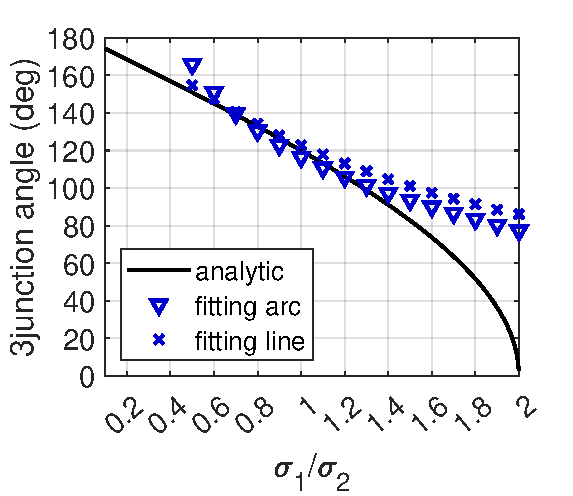
\includegraphics[width=\gwidth]{trijun_IWc_base.pdf}} ;
    \node[above right, inner sep=0] (trijun2) at (trijun1.south east)  {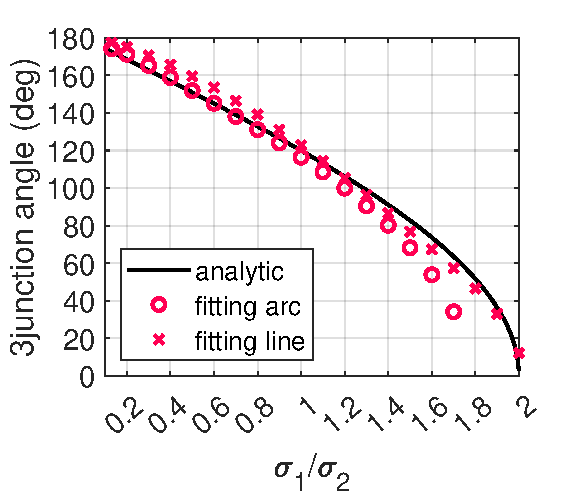
\includegraphics[width=\gwidth]{trijun_IWvG_base.pdf}};
    \node[above right, inner sep=0] (trijun3) at (trijun2.south east)  {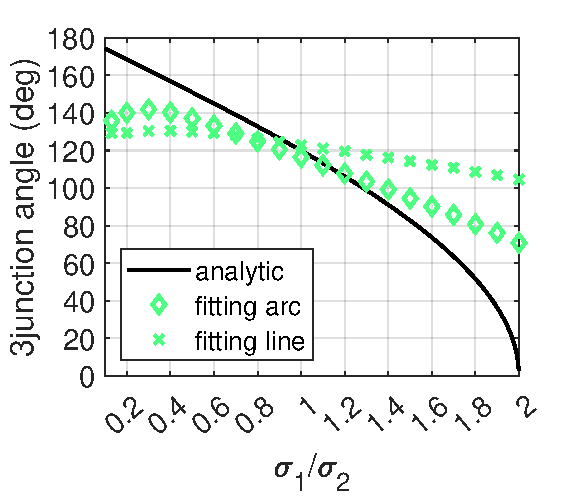
\includegraphics[width=\gwidth]{trijun_IWvK_base.pdf}};
    
    \draw[above, inner sep=0] (sketch.north west) node {(a)};
    \draw[above, inner sep=0] (trijun1.north west)+(0,-0.4) node {(b)};
    \draw[above, inner sep=0] (trijun2.north west)+(0,-0.4) node {(c)};
    \draw[above, inner sep=0] (trijun3.north west)+(0,-0.4) node {(d)};
\end{tikzpicture}
%% demo Wulff shapes
%\begin{tikzpicture}
%    \def\picwidth{0.2\textwidth};
%    \node[above right,inner sep=0] (i1) at (0,0)  {\includegraphics[width=\picwidth]{wulff/w_demomatch_O01.pdf}};
%    \node[above right,inner sep=0] (i6) at (i1.south east) {\includegraphics[width=\picwidth]{wulff/w_demomatch_O06.pdf} };
%    \node[below right,inner sep=0] (i3) at (i1.south west) {\includegraphics[width=\picwidth]{wulff/w_demomatch_O03.pdf} };
%    \node[above right,inner sep=0] (i8) at (i3.south east) {\includegraphics[width=\picwidth]{wulff/w_demomatch_O08.pdf} };
%    \node[below right,inner sep=0] (i5) at (i3.south west)  {\includegraphics[width=\picwidth]{wulff/w_demomatch_O05.pdf}};
%    \node[above right,inner sep=0] (i10) at (i5.south east) {\includegraphics[width=\picwidth]{wulff/w_demomatch_O10.pdf} };
%    
%    \foreach \piclab/\n/\Omg/\model in {(a)/1/0.2/IWc, (d)/6/2.3/IWvK, (b)/3/0.6/IWvK, (e)/8/4.9/IWvG, (c)/5/1/IWvG, (f)/10/7.5/IWc}
%    {
%        \draw[above,inner sep=0] (i\n.south) node {\piclab~\model, $\Omega=$\Omg};
%    }
%\end{tikzpicture}
%% Wulff shape match base
%\begin{tikzpicture}
%    \def\picwidth{0.49\textwidth};
%    \node[above right,inner sep=0] (i1) at (0,0)  {\includegraphics[width=\picwidth]{wulff/w_match_base.pdf}};
%    \node[below right,inner sep=0] (i2) at (i1.south west) {\includegraphics[width=\picwidth]{wulff/w_shape_corner_O10_base_1070_1080_1090.pdf} };
%    
%    \draw[above, inner sep=0] (i1.north west)+(0,-0.4) node {(a)};
%    \draw[above, inner sep=0] (i2.north west)+(0,-0.4) node {(b)};
%\end{tikzpicture}
%% Wulff shape shrinkage rate
%\begin{tikzpicture}
%    \node[above right,inner sep=0] (i1) at (0,0)  {\includegraphics[width=0.49\textwidth]{wulff/w_shrrate_base.pdf}};
%    \node[below right,inner sep=0] (i2) at (i1.south west) {\includegraphics[width=0.23\textwidth]{wulff/w_shrrate_O10_base_1070_1080_1090.pdf} };
%    \node[above right,inner sep=0] (i3) at (i2.south east) {\includegraphics[width=0.23\textwidth]{wulff/w_shrrate_O10_IWhalf_1100_1110_1120.pdf} };
%    
%    \draw[above, inner sep=0] (i1.north west)+(0,-0.4) node {(a)};
%    \draw[above, inner sep=0] (i2.north west)+(0,-0.4) node {(b)};
%    \draw[above, inner sep=0] (i3.north west)+(0,-0.4) node {(c)};
%\end{tikzpicture}
%%  companiso
%\begin{tikzpicture}
%    \node[above right,inner sep=0] (i1) at (0,0)  {\includegraphics[width=0.49\textwidth]{companiso/companiso_circmatch_base_fullaniso_reg.pdf}};
%    \node[below right,inner sep=0] (i2) at (i1.south west)  {\includegraphics[width=0.49\textwidth]{companiso/companiso_relshrrate_base_fullaniso_reg.pdf}};
%    \node[below right,inner sep=0] (i3) at (i2.south west) {\includegraphics[width=0.23\textwidth]{companiso/companiso_shrrate_O5_base_fullaniso_reg_115_120_125.pdf}};
%    \node[above right,inner sep=0] (i4) at (i3.south east) {\includegraphics[width=0.23\textwidth]{companiso/companiso_shrrate_O5_14IWpts_fullaniso_reg_130_135_140.pdf} };
%    
%    \draw[above, inner sep=0] (i1.north west)+(0,-0.4) node {(a)};
%    \draw[above, inner sep=0] (i2.north west)+(0,-0.4) node {(b)};
%    \draw[above, inner sep=0] (i3.north west)+(0,-0.4) node {(c)};
%    \draw[above, inner sep=0] (i4.north west)+(0,-0.4) node {(d)};
%\end{tikzpicture}
%% INITIAL CONDITIONS - SKETCHES
%\begin{tikzpicture}
%    \node [above right, inner sep=0] (img1) at (0,0) {\includegraphics[page=3,width=0.23\textwidth ]{Sketches.pdf}};
%    \node [below right, inner sep=0] (img2) at (img1.north east) {\includegraphics[page=4,width=0.23\textwidth ]{Sketches.pdf}};
%    
%    \draw[above, inner sep=0] (img1.north west)+(0,-0.6) node {(a)};
%    \draw[above, inner sep=0] (img2.north west)+(0,-0.6) node {(b)};
%    
%    % \node [below right, inner sep=0] (img3) at (img1.south west) {\includegraphics[page=1,width=0.23\textwidth]{Sketches.pdf}};
%    % \node [below right, inner sep=0] (img4) at (img3.north east) {\includegraphics[page=2,width=0.23\textwidth]{Sketches.pdf}};
%    \node [below, inner sep=0] (img4) at (img1.south east) {\includegraphics[page=2,width=0.23\textwidth]{Sketches.pdf}};
%    
%    % \draw[above, inner sep=0] (img3.north west)+(0,-0.6) node {(c)};
%    \draw[above, inner sep=0] (img4.north west)+(0,-0.6) node {(c)};
%\end{tikzpicture}
\end{document}
